\documentclass{DGC_M2_report}
 
\RequirePackage{pslatex}
\usepackage{charter}
\usepackage[utf8]{inputenc}
\usepackage[T1]{fontenc}
\usepackage[francais]{babel}
\usepackage[top=2cm, bottom=2cm, left=2cm, right=2cm]{geometry}
\usepackage{amsmath}
\usepackage{amssymb}
\usepackage{mathrsfs}
\usepackage{graphicx}
\usepackage{color} 
\usepackage{colortbl}
\usepackage{slashbox}
                           
%\title{FISSURATION D'ELEMENTS EN BETON ET EFFETS D'ECHELLE}
%\author{Christian \textsc{Nader}\\Encadrement: \textsc{C. Olivier-Leblond,C. Giry, F. Ragueneau}}
%\date{\\Le 20 Juin 2013} 

\graphicspath{{figures/}}
\hypersetup{%
   pdftitle    = {Rapport de stage M2},
   pdfsubject  = {Rapport},
   pdfauthor   = {christian NADER},
   pdfkeywords = {mots, clés}}

 
\begin{document}
  
%\maketitle
\thispagestyle{empty}
\enlargethispage{1cm}\vspace*{-2cm}
\begin{center}\normalfont\bfseries


\noindent
\includegraphics[height=1.6cm]{LogoENS}
\hfill

\includegraphics[height=1.6cm]{LogoUPMC}
\hfill
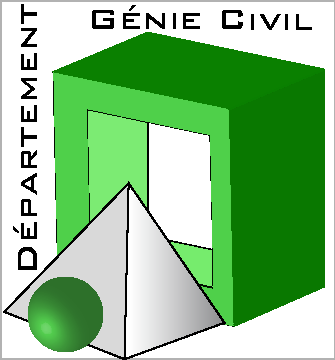
\includegraphics[height=2.3cm]{LogoDGC}

\par\vspace{.25cm}  Master  Sciences de l'Ing�nieur, Sp�cialit� G�nie Civil  \par  Parcours  Structures, Ouvrages et
Mat�riaux du G�nie Civil\\
  \rule{\linewidth}{.25mm}


\par\vspace{1cm}  \textnormal{\bfseries MEMOIRE DE STAGE DE MASTER 2\up{e} ANNEE}

\par\vspace{.25cm} \textnormal{effectu� au LMT Cachan}
\par\textnormal{sous la direction de C. Oliver-Leblond, C. Giry, F. Ragueneau}


\par\vspace{\stretch{0.5}} \textnormal{\bfseries\Large FISSURATION D'ELEMENTS EN BETON ET EFFETS D'ECHELLE}
\par\vspace{.5cm} {\bfseries par}
\par\vspace{.5cm}\textnormal{\bfseries\Large Christian NADER}

\par\vspace{\stretch{1}}
   \rule{\linewidth}{.25mm}
\par\textnormal{Soutenu � l'ENS Cachan le 28 juin 2013}
\par\textnormal{61 avenue du Pr�sident Wilson, F-94235 Cachan cedex, France}
\end{center}
\clearemptydoublepage


\chapter*{Remerciements}
thank you thank you've been a great audience

\renewcommand{\contentsname}{Sommaire} 
\tableofcontents 
\listoffigures

\chapter*{Introduction}
\addcontentsline{toc}{chapter}{Introduction} 
Dans ce stage on propose un protocole expérimental permettant de mettre en œuvre des essais de
flexion sur poutre en béton mettant en évidence des effets d'échelle en termes de fissuration.
Les résultats de l'étude faite sur des poutres en micro-béton entaillées et non entaillées
chargées en flexion trois points seront comparés à d'autres résultats expérimentaux et les lois
d'effet d'échelle de Bažant. On confirme déjà l'existence de l'effet d'échelle sur des poutres de
petites tailles (ce qui est le cas de notre étude). Cependant, pour de plus grandes poutres non
entaillées la résistance nominale tend vers une valeur constante liée à la résistance en traction
uniaxiale. Il a été conclu que l'applicabilité de la loi d'effet d'échelle dépend du type de
problème, ceci dit, si la propagation de la fissure avant la charge ultime est très stable, la loi
d'effet d'échelle peut être utilisée dans une gamme de taille plutôt large. Toutefois, si ce n'est pas
le cas, la validité de la loi d'effet d'échelle est limitée à une plage de taille plus petite. Par
conséquent, on ne peut pas extrapoler l'effet d'échelle à partir des essais avec une gamme de
taille petite à une gamme de grande taille, pour cela il nous manque des données expérimentales
provenant d'essais sur de gammes de grande taille. Ainsi, dans notre étude, nous allons négliger
cette partie de la problématique, puisque nous allons tester seulement de petites poutres, plutôt,
nous allons nous concentrer sur d'autres aspects de l'effet d'échelle tels que les propriétés de la
résistance nominale d'une structure contenant une entaille (ou initialement une grande fissure) et
d'autres initialement non entaillées.\\\\
Mots-clés: Flexion trois points, Béton, Fissure, Effet d'échelle


\part{Bibliographie}
\chapter{Effet d'échelle}
\section{Introduction}
L'effet d'échelle dans les matériaux quasi fragile comme le béton est un phénomène bien connu
et il existe un certain nombre d'études expérimentales et théoriques (Rusch et al, 1962; Leonhardt
et Walter, 1962; Kani, 1967; Bhal, 1968; Taylor, 1972; Walsh 1976: Walraven et Lehwalter
1990; Chana 1981; Reinhardt, 1981 a,b; Iguro et al, 1985; Hillerborg, 1989; E1igehausen et al.
1992) qui confirment l'existence de celui-ci. Il ya deux aspects de l'effet d'échelle : statistique et
déterministe. Basés sur la mécanique de la rupture. Dans le passé, l'effet d'échelle a été
principalement traitée du point de vue statistique (Weibull, 1939; Mihashi et Zaitscv, 1981;
Mihashi, 1983). Cependant, actuellement il ya suffisamment de preuves qui montent que la
raison principale de l'effet d'échelle réside dans la libération de l'énergie de déformation due à la
croissance de la rupture.\\\\
Selon Bažant (1984) l'effet d'échelle peut être approximativement décrit par la loi d'effet
d'échelle:\[\sigma_{N}=Bf_{t}(1+\beta)^{-1/2}  ; \beta=d/d_0\]
Où d est une mesure d'une taille caractéristique de la structure (par exemple hauteur de la
poutre), $f_t =$ résistance à la traction du béton, $B$ et $d_0$ sont deux constantes à déterminer, soit
expérimentalement, soit par une analyse plus sophistiquée. Selon l'équation au dessus la
résistance nominale $\sigma_N$ de grandes structures tend vers zéro et la charge de rupture augmente
avec $d$.\\\\
En supposant que les les propriétés du matériau sont constantes (le même béton), la
dérivation de la loi effet d'échelle repose sur quatre hypothèses de base: (1) La propagation d'une
fissure ou rupture nécessite une alimentation presque constante en énergie par unité de longueur
et largeur ($G_F$, énergie de fissuration du béton, indépendante de la taille de l'échantillon) (2)
l'énergie libérée par la structure en raison de croissance de la rupture est une fonction à la fois de
la longueur de rupture et la surface de la zone de fissuration (FPS, Fracture Process Zone) à
l'avant de la fissure. Si la libération d'énergie potentielle est une fonction de la longueur de la
fissure seulement, l'effet d'échelle est celui de la LEFM (Linear Elastic Fracture Mechanics), et
si elle est fonction de la zone de rupture seule, il n'y a pas d'effet d'échelle. (3) À la charge
limite, les formes et longueurs des fissures dans les structures géométriquement semblables de
différentes tailles sont également géométriquement semblables, et (4) la structure ne casse pas à
l'amorçage de la fissure, en d'autre termes, la propagation de la fissure doit être possible.

\section{Loi en puissance}
C'est la base mathématique qui va nous donner la forme des équations qui gèrent les effets d'échelle.\\\\   
Cherchons à déduire une réponse $Y$ comme fonction de la dimension
caractéristique $D$ d'une structure. Imaginons maintenant des structures de trois dimensions $D_0$, $D_1$ et $D$, avec les réponses correspondantes $Y_0$,$Y_1$ et $Y$. Etant donné qu'il n'y a pas de longueur
caractéristique, on cherche la fonction adimensionnelle $f(\lambda)$ avec $\lambda = \frac{D}{D_0}$, et $\frac{Y}{Y_0} = f(\lambda)$ ; $D_0$ est pris comme dimension de référence, cela implique que $\frac{Y_1}{Y_0} = f(\frac{D_1}{D_0})$.
Ainsi, \[\frac{Y}{Y_1} = \frac{f(\lambda)}{f(\frac{D_1}{D_0})}\]
Et si il n'y a pas de longueur caractéristique, on peut écrire ce qui suit: $\frac{Y}{Y_1} = f(\frac{D}{D_1})$, ce qui implique la condition:
\[\frac{f(\frac{D}{D_0})}{f(\frac{D_1}{D_0})} = f(\frac{D}{D_1})\]
On doit la différencier par rapport à $D$ (la seul variable dans le système), ce qui donne:\[\frac{1}{f(\frac{D_1}{D_0})}.\frac{df}{dD}(\frac{D}{D_0}).\frac{1}{D_0} = \frac{df}{dD}(\frac{D}{D_1}).\frac{1}{D_1}\]
Pour $D_1 = D$ et $\frac{dD}{dD} = \frac{d\lambda}{d\lambda}$ on obtient:
\[\frac{1}{f(\frac{D}{D_0})}.df(\frac{D}{D_0}) = \frac{df}{dD}(\frac{D}{D}).\frac{dD}{D_1}D_0\]
Par suite \[\frac{df(\lambda)}{f(\lambda} = m.\frac{d\lambda}{\lambda}\text{  ; avec  }m = \frac{df(1)}{d\lambda}\]
Finalement ,sa primitive ,avec la condition $f(1) = 1$, donne: \[\ln(f(\lambda)) = m.\ln(\lambda) = \ln(\lambda^m)\]
D'où l'effet d'échelle en puissance: $f(\lambda) = \lambda^m$ (on démontre par intégrale $J$ que $m = -1/2$)



\section{Analyse asymptotique dans les poutres entaillées}
La fissuration peut être caractérisée
par les variables adimensionnelles $\alpha_0 = \frac{a_0}{D}$, $\alpha = \frac{a}{D}$, $\theta = \frac{c_f}{D}$, dans lesquelles \og$a$\fg{} c'est la longueur équivalente de fissure qui donne la même complaisance que le système avec sa fissure réelle et
avec sa zone d'élaboration ; $c_f=a-a_0$ taille effective de la zone d'élaboration de la fissuration.
\\
\begin{center}
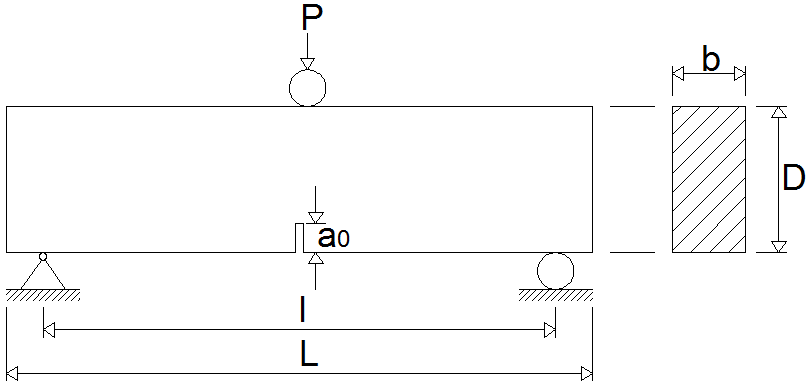
\includegraphics[scale=0.5]{figure1}
\end{center}
\\\\
L'énergie restituée par la structure peut être analysée sur la base de la variation de
l'énergie complémentaire de la structure: $\Pi^* = \sigma_{N}^{2}.b.D^2/E.f(\alpha_0, \alpha, \theta)$ ; ici '$f$' est une fonction adimentionnelle caractérisant la géométrie de la structure. D'autre part, la résistance à la
fissuration peut être caractérisée comme $R=G_f.r(\alpha_0, \alpha, \theta)$, où '$r$' est une autre donction adimentionnelle ayant la propriété que $\lim_{\alpha \to \alpha_0} r = 1$.\\\\
On déduit ainsi le taux de restitution d'énergie $G = (\frac{d\Pi^*}{d\alpha})/b$, et pour un $\sigma_N$ constant on peut écrire le suivant: $\frac{dG}{d\alpha} = \frac{dR}{d\alpha}$
\\\\
On peut montrer à partir des équations précédentes que la résistance nominale de la
structure est donnée sous la forme: \[\sigma_N = \sqrt{\frac{E.G_f}{D.g(\alpha_0, \theta)}}\]
où ‘$g$' est une fonction adimensionnelle
exprimée en termes des fonctions ‘$f$' et ‘$r$' et leurs dérivées.
\\\\
La fonction ‘$g$' doit être régulière, et donc par développement en série de Taylor jusqu'au $2^{nd}$ ordre au voisinage de $(\alpha_0, 0)$ on aura:
\[\sigma_N = \sqrt{\frac{E.G_f}{D}}.(g(\alpha_0, 0)+g_1(\alpha_0, 0).\frac{c_f}{D}+...)^{-1/2}\]
Par conséquent, l'analyse de l'effet d'échelle à l'aide du taux de restitution d'énergie est possible par l'introduction de l'approximation $g(\alpha_0, \theta) = g(\alpha_0 + \theta)$, on obtient ainsi:
\begin{equation}
\sigma_N = \sqrt{\frac{E.G_f}{c_f.g'(\alpha_0)+D.g(\alpha_0)}} = B.f'_{t}(1+\frac{D}{D_0})^{-1/2}
\end{equation}
dans laquelle les paramètres sont donnés par: $D_0 = c_f.\frac{g'(\alpha_0)}{g(\alpha_0)}$, $B.f'_{t}=\sqrt{\frac{E.G_f}{c_f.g'(\alpha_0)}}$



\section{Effet d'échelle à l'amorcage de la fissure}
En dehors des éprouvettes entaillées,
l'analyse précédente ne s'applique qu'aux structures qui contiennent, à la charge maximale, une
grande fissure. La ruine à l'amorçage de la fissuration à partir d'une surface plane (éprouvette
non entaillée) peut aussi être analysée sur la base des développements à partir des équations
précédentes, avec, cependant, une modification. Puisque les développements sont faits par
rapport à une valeur nulle de la taille de la zone d'élaboration relative, l'argument de la fonction
de restitution d'énergie $g(\alpha)$ est $\alpha=0$, ce qui signifie que le taux de restitution d'énergie
$g(\alpha)=g(0)=0$. Dès lors, le premier terme du développement aux grandes tailles disparait, il faut
dans ce cas inclure le troisième terme du développement asymptotique aux grandes tailles. Ce
qui conduit à l'approximation suivante de la résistance nominale de structures dont la ruine
apparait dès l'amorçage de la fissuration à partir d'une surface plane:
\begin{equation}
\sigma_N = \sqrt{\frac{E.G_f}{c_f.g'(\alpha_0)+\frac{1}{2}.g''(\alpha_0).c_{f}^{2} .D^{-1}}}
\end{equation}
Pour présenter l'effet d'échelle de façon plus détaillée, le comportement des poutres en
micro-béton, entaillées et non entaillée, chargées en flexion trois points, sera étudié.



\section{Effet d'echelle en flexion trois points}
Dans la littérature, un certain nombre de résultats d'essai pour des poutres avec et sans entaille,
testées en flexion trois points, spécimens ont été rapportés. Dans la Fig. 1, résultats d'essais pour
trois spécimens de poutres entaillées mis à l'échelle (ratio taille d'entaille - hauteur de la poutre,
$\frac{a_0}{d} = \frac{1}{6}$), réalisées à Northwestern University (Bazant et Pfeiffer, 1987), sont présentés. Dans
la même figure on compare ces résultats avec les résultats numériques (Eligehausen et Oiboll,
1992) et la loi d'effet d'échelle. La profondeur des poutres a été modifié dans une plage de taille
assez faible, soit de $d = 76 mm$ à $305 mm$ avec une épaisseur constante $b = 38 mm$. La résistance
nominale à la rupture est calculée en utilisant la formule de la théorie des poutres $\sigma_N = \frac{15P.U}{4b.d}$
avec Pu étant la charge ultime. D'après la Fig. 1, un effet d'échelle significative est observé, la
résistance nominale σN diminue avec l'augmentation de la taille. La loi effet de taille est en
accord avec les résultats expérimentaux.
\begin{center}
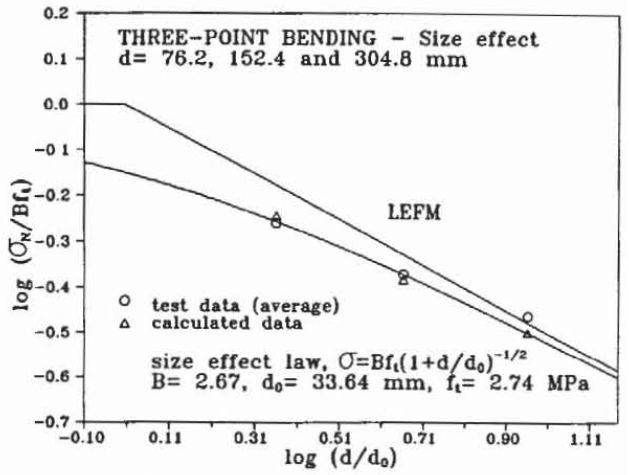
\includegraphics[scale=0.65]{Fig_1}
\end{center}
\begin{center}
\caption{Fig.1 Effet d'échelle en flexion trois points sur des poutres entaillées ($a_0/d=1/6$)}
\end{center}
Les résultats des essais rapportés par Malkov et Karavaev (1968) et Heilmann (1969)
pour des échantillons non entaillées en béton ordinaire en flexion trois points sont représentés sur
la Fig. 2. La plage de hauteur de la poutre était jusqu'à $1000 mm$. Comme on peut le voir sur la
figure 2, les résultats des tests jusqu'à une profondeur de la poutre d'environ $d = 500 mm$
présentent un effet d'échelle significative en accord relativement avec la loi d'effet d'échelle.
Cependant, pour les plus grands spécimens, la résistance nominale tend à la résistance en traction
uniaxiale du béton.
\begin{center}
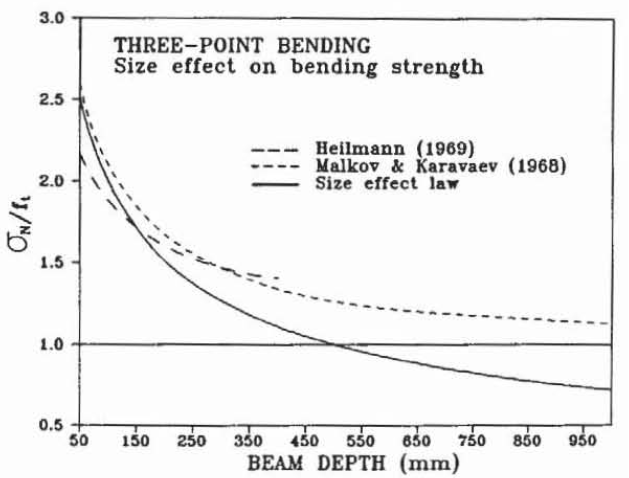
\includegraphics[scale=0.65]{Fig_2}
\end{center}
\begin{center}
\caption{Fig.2 Effet d'échelle en flexion trois points sur des poutres non entaillées}
\end{center}
Dans la Fig. 3 la résistance nominale des poutres avec une taille constante d'entailles,
testés par Alexander (1987) sont tracés en fonction de la hauteur. Comme dans le cas des
éprouvettes non entaillées, la résistance nominale des grandes poutres tend vers une valeur
cte différente de $0$.
\begin{center}
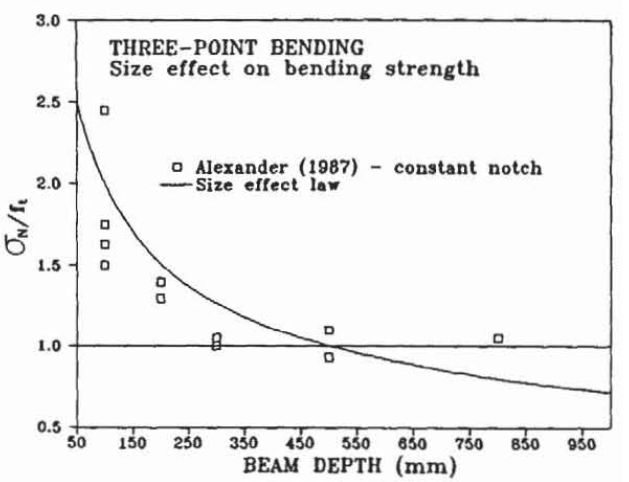
\includegraphics[scale=0.65]{Fig_3}
\end{center}
\begin{center}
\caption{Fig.3 Effet d'échelle en flexion trois points sur des poutres entaillées (même taille d'entaille)}
\end{center}



\chapter{Energie de fissuration}
\section{Taux de restitution d'energie}
\og La puissance mécanique disponible pour ouvrir une fissure de surface $A$ est égale à la variation de l'énergie totale $V$, appelée \emph{taux de restitution d'énergie}\fg{}(unité: $joule/m^2$):
\[G=\trac{\partial V}{\partial A}\]
\begin{itemize}
\item propagation de la fissure si: $G-2\gamma^s \geq 0$
\item arrêt si: {} {} {} {} {} {} {} {} {} {} {} {} {} {} {} {} {} {} {} {} {} {} {} {} {} {} {} {} {} {} {} $G-2\gamma^s \leq 0$
\end{itemize}
avec $\gamma^s$ énergie spécifique de rupture par unité de surface\\
Après son amorçage, la fissure s'arrête, nécessitant plus d'énergie pour reprendre sa propagation (en déplacement imposé, la propagation de la fissure est presque toujours stable).


\section{Méthode de détermination}
L'énergie de rupture Gf qui est obtenu par cette méthode est définie comme l'énergie spécifique
(énergie par unité de zone plane de fissuration) nécessaire pour la croissance de fracture dans un
échantillon d'essai infiniment grand. La méthode est décrite ici pour le mode I de rupture
uniquement. Les résultats des tests dont on a besoin pour déterminer l'énergie de rupture ne sont
que les valeurs de la charge maximale $P_1$, $P_2$, $P_3$ pour les spécimens de différents tailles, $D_1$,
$D_2$, $D_3$, et le module de Young du béton, $E$. Le module de Young peut être obtenu en utilisant
toute autre méthode conventionnelle, par exemple, essais de compression sur des échantillons cylindriques.
\\\\
Procédure de calcul: Les charges maximales corrigées qui prennent le poids de
l'échantillon en compte: $P_{j}^{0} = P_j + \frac{1}{2}m_j.g$, dans laquelle $m_j$ est la masse du spécimen $j$, $g$ est l'accélération de la pesanteur.
\\\\
On effectue maintenant une régression linéaire, compte tenu du tracé des ordonnées $Y_j$ contre les abscisses $X_j$ où: $Y_j = (b.d_j/P_{j}^{0})^2$, $X_j = d_j$
\\
Interception de la droite de régression : $Y = AX + C$, avec
\[A=\frac{\sum_{j} (X_j-\overline{X})(Y_j-\overline{Y})}{\sum_{j} (X_j-\overline{X})^2} \text{{  };{  }} C=\overline{Y}-A\overline{X} \text{{  };{  }} \overline{X}=\frac{1}{n}\sum_{j}X_j \text{{  };{  }} \overline{Y}=\frac{1}{n}\sum_{j}Y_j\]
Calcul des valeurs auxiliaires pour l'extrapolation : pour $l/d = 4$ (comme notre cas)
\[F_4(\alpha)=\frac{1.99-\alpha(1-\alpha)(2.15-3.93\alpha+2.7\alpha^2)}{\pi^{1/2}(1+2\alpha)(1-\alpha)^{3/2}}\]
Energie libérée:
\[g(\alpha)=(\frac{l}{d})^2\pi\alpha(1.5F(\alpha))^2\]
Energie de fissuration:
\[G_f=\frac{g(\alpha_0)}{E_cA}\]
Statistique:
\[S_{x}^{2}=\frac{1}{n-1}\sum_{j} (X_j-\overline{X})^2\text{ ; }S_{y}^{2}=\frac{1}{n-1}\sum_{j} (Y_j-\overline{Y})^2\text{ ; }S_{y|x}^{2}=\frac{1}{n-2}\sum_{j} (Y_{j}-Y'_j)^{2}=\frac{n-1}{n-2}(S_{y}^{2}-A^2S_{x}^{2})\]
\[w_{y|x}=S_{y|x}\overline{Y}\text{ ; }w_x=S_x\overline{X}\text{ ; }w_A=\frac{S_{y|x}}{AS_x(n-1)^{1/2}}\]
\[w_C=\frac{S_{y|x}}{C(n-1)^{1/2}}(1+\frac{1}{w_{x}^{2}})^{1/2}\text{ ; }m=\frac{w_{y|x}}{w_x}\]
On prend comme approximation : $w_{G}^{2}=w_{A}^{2}+w_{E}^{2}$, avec $w_E$: coef de variation de $E_c$


\chapter{correlation d'image}
\section{Introduction}
La méthode de corrélation d'images numériques a été créé comme un outil stable et fiable pour la
mesure des fractures / dommages (Lawler, Keane, et Shah, 2001; Luo Chao, Sutton, & Peters,
1993; Shah, Swartz, & Ouyang, 1995). La méthode de corrélation d'images a été fréquemment
utilisée pour l'étude du mode d'ouverture de la rupture de matériaux quasi-fragiles comme le
béton (Choi et Shah, 1997). Dans les travaux de Choi et Shah (1997), la précision de mesure de
déplacement a été estimée à l'aide de trois procédures différentes et l'erreur maximale a été
trouvée à environ $1/20$ pixels. Il a été constaté que la corrélation d'images est très efficace pour
déterminer la largeur des fissures et l'emplacement des petites fissures.
Contrairement aux méthodes plus traditionnelles, la corrélation d'images est une
technique robuste avec un degré élevé de précision de mesure, et elle est beaucoup plus facile à
appliquer expérimentalement. Le processus de corrélation consiste de capturé la surface de
l'échantillon ayant des modes distribués de niveau de gris. L'efficacité du modèle de speckle peut
être déterminée à partir de la quantité de pixels par speckle noir. Ces schémas, l'un avant et
l'autre après la mise en charge, sont imagés par un appareil photo numérique et stockées dans un
ordinateur dans un format digital. Pendant le processus de formation d'image, l'intensité de la
configuration aléatoire est transformée en un nombre fini d'échantillons sur une grille
rectangulaire. Chaque capteur, ou pixel, dans une caméra typique moyenne l'intensité de la
lumière incidente sous la forme d'une valeur d'intensité de gris, qui est normalement dans
l'intervalle de $0-256$ (on peut allez plus loin dans la précision en partant avec des photos de haute qualités en \emph{RAW} (image brute) et les convertires de façon à concerver la particularité de notre gris, on obtient dans ce cas un spectre qui peut contenir $16000$ valeurs! ; cette méthode est bien sûre plus compliqué et prend trops de temps).

\section{Principe}
Traitons deux images, qui caractérisent la surface initiale et déformée d'un
matériau soumis à une charge connue. Une image est une fonction scalaire de la coordonnée
spatiale qui donne le niveau de gris de chaque point discret (ou pixel) de coordonnée x. Les
images de la référence et états déformés sont appelés respectivement $f(x)$ et $g(x)$. Soit $u(x)$ le
champ de déplacement. Ce champ permet de relier les deux images en exigeant la conservation
du flux optique
\[g(x)=f(x+u(x))\]
En supposant que l'image de référence est différentiable, un développement de Taylor au premier
ordre donne
\[g(x)=f(x)+u(x).\bigtriangledown f(x)\]
\begin{center}
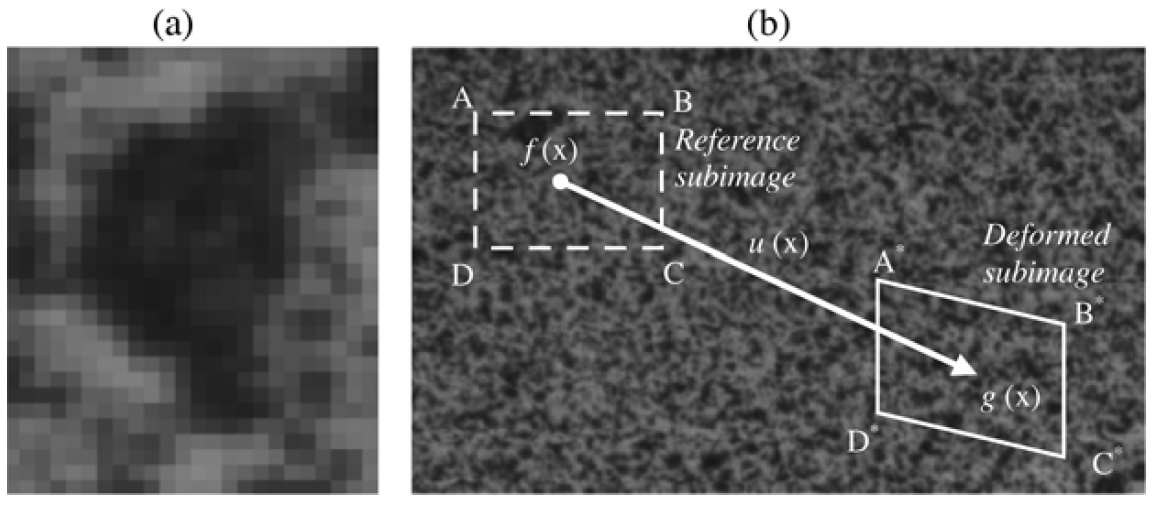
\includegraphics[scale=0.5]{Fig_4}
\end{center}
\begin{center}
\caption{Fig.4 (a) Zoom sur un motif moucheté. Le modèle speckle est d'environ $15\times 20$ pixels. (b) Représentation schématique de la déformé et l'image de référence situés sur une photo instantanée.}
\end{center}
Ensuite, par minimisation on obtient une fonction objective, et en considérant $u(x)$ comme
la somme de fonctions scalaires, la minimisation nous donne alors un system linéaire qui
ressemble à la relation suivante:
\[M.a=b\]
Avec
\[u(x)=\sum_{\alpha,n} a_{\alpha n}\psi_n(x)e_\alpha \]
\[M_{\alpha n \beta m}=\int{\int_{\Omega} {[\psi_m(x)\psi_n(x)\partial_\alpha f(x)\partial_\beta f(x)]\ dx}}\]
\[b_{\alpha n}=\int{\int{[g(x)-f(x)]\psi_n(x)\partial_\alpha f(x)\ dx}}\]

\section{Discrétisation par éléments finis (Correli $Q4$)}
Puisque l'image est naturellement divisée en pixels, il
convient de choisir une forme carrée ou rectangulaire pour chaque élément. Ce qui nous amène
au choix d'éléments finis type $Q4$ comme base la plus simple. Chaque élément est associé sur le
carré $[0 ; 1]^2$, où les quatre fonctions de base sont $(1-x)(1-y)$, $x(1-y)$, $(1-x)y$ et $xy$ dans un repère
$(x ; y)$ local. La décomposition de déplacement est donc particularisée pour tenir compte des
fonctions de forme d'une discrétisation par éléments finis.
\[u^e(x)=\sum_{n=1}^{n_e} \sum_{\alpha} a_{\alpha n}^{e}N_n(x)e_\alpha\]
Où $n_e$ est le nombre de noeuds (ici $n_e = 4$), et '$a$', les déplacements nodaux inconnus. La
fonction objective est alors reformulée, on obtient la forme discrétisé de la matrice $M$ et du
vecteur $b$
\[M_{\alpha n \beta m}^{e}=\int{\int_{\Omega_e} {[N_m(x)N_n(x)\partial_\alpha f(x)\partial_\beta f(x)]\ dx}}\]
\[b_{\alpha n}^{e}=\int{\int{[g(x)-f(x)]N_n(x)\partial_\alpha f(x)\ dx}}\]
Ainsi, il devient possible de calculer pour chaque élément '$e$' les contributions élémentaires
de $M$ et $b$.


\part{Procédure expérimentale}
\chapter*{}
Cette section est consacrée à la présentation de la campagne expérimentale menée sur des
poutres homothétiques, entaillées et non-entaillées faites du même matériau. Nous avons
considéré trois géométries différentes afin de prendre en compte les effets d'échelle et les effets
de bord.



\chapter{Les échantillons}
\section{Description du matériau}
Dans notre étude on test des éprouvettes de petites dimensions on a alors recours à utiliser un
micro-béton. (Référence: rapport de stage de Amine Hamouche - 2010)
\\\\
La composition du micro-béton pour $1m^3$ est présenté dans le tableau 1. Le ciment utilisé
est un CEM1 $52,5 N$ (HOLCIM), et le sable normalisé est conforme $ISO  679$, sa granulométrie
est $0/2 mm$ et donnée dans le tableau 2. Le rapport $e/c$ est de $0,46$. Cette formulation est tirée de
la thèse de Anna Ouglova 2004.

\begin{table}[h]
\begin{center}
\begin{tabular}{ccc}
\hline
\begin{bf}                   Sable(Kg)         \end{bf} & \begin{bf}                   Eau(Kg)         \end{bf} & \begin{bf}                   Ciment(Kg)           \end{bf} \\
\hline 
\begin{bf}\rowcolor{cyan}1342\end{bf} & \begin{bf}294\end{bf} & \begin{bf}631\end{bf} \\
\hline 
\end{tabular}
\end{center}
\caption{Composition du micro-béton}
\label{micro-béton}
\end{table}
\begin{table}[h]
\begin{center}
\begin{tabular}{cc}
\hline
\begin{bf}Tamis ouverture des mailles (mm)\end{bf}   &   \begin{bf}refus cummulés (\%)\end{bf} \\
\hline 
\begin{bf}\rowcolor{cyan}0.08\end{bf}   &   \begin{bf}99 \pm{}1 \end{bf} \\ 
\begin{bf}0.16\end{bf}   &   \begin{bf}87 \pm{}5\end{bf} \\
\begin{bf}\rowcolor{cyan}0.50\end{bf}   &   \begin{bf}67 \pm{}5\end{bf} \\
\begin{bf}1.00\end{bf}   &   \begin{bf}33 \pm{}5\end{bf} \\
\begin{bf}\rowcolor{cyan}1.60\end{bf}   &   \begin{bf}7 \pm{}5\end{bf} \\
\begin{bf}2.00\end{bf}   &   \begin{bf}0\end{bf} \\
\hline 
\end{tabular}
\end{center}
\caption{Granulométrie du sable normalisé}
\label{sable}
\end{table}



\section{Géométrie des éprouvettes}
Les essais de flexion seront réalisés sur des poutres de dimensions $B\times D\times L{} cm^3 (largeur \times{} hauteur
\times{} longueur)$ avec un rapport $L/D=5$ constant et $B$ une dimension fixe (restriction du type de test,
ici $B=4 cm$).
\\\\
Trois différentes tailles sont considérées, présentant toutes un rapport $L/D = 5$, où $L$ est la
longueur et $D$ est la hauteur de la poutre. La profondeur, quant à elle a été choisie constante et
égale à $B (4 cm)$. Les entailles centrales seront taillées après coulage et non moulées sur les
éprouvettes. Trois longueurs d’entaille ont été considérées avec une épaisseur d’entaille
constante de $2 mm$ pour tous les échantillons (voir figure 4, page suivante).
\\\\
On propose les dimensions suivantes :
\begin{table}[h]
\begin{center}
\begin{tabular}{c|c|c|c|c}
\hline
\backslashbox{\begin{bf}taille\end{bf}}{\begin{bf}dimension\end{bf}}   &   \begin{bf}épaisseur\end{bf}   &   \begin{bf}hauteur\end{bf}   &   \begin{bf}longueur\end{bf}   &   \begin{bf}distance entre appuis\end{bf}\\
\hline
 
\begin{bf}\rowcolor{cyan}$n_1$\end{bf}   &   \begin{bf}$B_1=4cm$\end{bf}   &   \begin{bf}$D_1=4cm$\end{bf}   &   \begin{bf}$L_1=20cm$\end{bf}   &   \begin{bf}$I_1=16cm$\end{bf} \\

\begin{bf}$n_2$\end{bf}   &   \begin{bf}$B_2=4cm$\end{bf}   &   \begin{bf}$D_2=8cm$\end{bf}   &   \begin{bf}$L_2=40cm$\end{bf}   &   \begin{bf}$I_2=32cm$\end{bf} \\

\begin{bf}\rowcolor{cyan}$n_3$\end{bf}   &   \begin{bf}$B_3=4cm$\end{bf}   &   \begin{bf}$D_3=8cm$\end{bf}   &   \begin{bf}$L_3=80cm$\end{bf}   &   \begin{bf}$I_3=64cm$\end{bf} \\

\hline 
\end{tabular}
\end{center}
\caption{Les dimensions des éprouvettes}
\label{sable}
\end{table}

%%%%%%%%%%%%%%%%%%%%%%%%%%%%%%%%%%%%%%%%%%%%%%%%%%%%%


\section{Coffrages}
Types de bois :\\
\begin{itemize}
\item[•] bois standard (BS, joue le rôle de support)
\item[•] bois de coffrage (BC, en contact avec le béton)\\
\end{itemize}
Pour concevoir le coffrage on utilise des planches de bois standard de $2,5m \times{} 1,25m$
(épaisseur $1,5 cm$), ainsi que des planches de bois de coffrage de $2,5m \times{} 1,22m$ (épaisseur $1,8 cm$), on admet $4 mm$ comme trait de coupe.
\\\\
Les coffres seront conçus d’une façon à être réutilisables, on aura besoin alors de tiges
filetés ($2$ par éprouvette).
\\\\
On a besoin de $9$ coffres en total mais les coffres des éprouvettes qui ont une même09088
dimension seront exactement pareils.
\\
\begin{itemize}
\item[•] Pour les éprouvettes de dimension $4\times 4\times 20$ on peut faire un seul coffre de la manière
suivante : (N.B. : masse du coffre avec béton environ $6,5Kg$)
\end{itemize}




\section{Matériel et équipement}
Composants du micro-béton (perte 15\%) :\\
Volume total de béton :\\
\begin{itemize} 
\item[\triangleright] $27$ éprouvettes (poutres) : $v_1 = 60480 cm^3$
\item[\triangleright] $12$ échantillons cylindriques ($11\times 22$) pour définir les caractéristiques du béton (6 pour le
   test de compression uni-axial, 6 pour l’essai brésilien) : $v_2 = 25090 cm^3$
\item[\triangleright] $+5L$ (cône d’Abrams) $+1L$ (Aréomètre) : $v_3 = 6000 cm^3$
\item[\triangleright] Volume total : $V = 91570 cm^3$
\item[\triangleright] $+pertes$ : $V_{final} = 0.1053055 m^3$\\
\end{itemize}
Ainsi,d’après le Tableau -1- on peut calculer les quantités des composantes du béton:\\
\begin{itemize}
\item[•] Sable : $141.32 Kg$
\item[•] Eau : $30.96 Kg$
\item[•] Eau : Ciment : $66.45 Kg$\\
\end{itemize}
Matériels pour le coffrage :\\
\begin{itemize}
\item[•] Une plaque de bois standard
\item[•] Une plaque de bois de coffrage
\item[•] 16 écrous
\item[•] 16 rondelles
\end{itemize}





\chapter{Essai F3P}
\section{MTS}


\section{Pilotage}

\part{Étude numériques}
\chapter*{}
Dans notre étude on utilise comme matériau un micro-béton. Pour bien prédire numériquement
les résultats de l'expérience, on a besoin d'introduire les paramètres qui correspondes à ce
matériau, or par manque de données sur certains de ces paramètres (principalement la fragilité en
traction) on a recours à une identification par rapport à des essais expérimentaux. Pour cela on a
lancé plusieurs calcules sur des échantillons similaires aux échantillons de l'expérience en
géométrie et chargement et on a changé les paramètres d'une façon intuitive pour obtenir au final
une courbe force/déplacement similaire aux courbes trouvées expérimentalement.

\chapter{Modélisation}
\section{Mode de calcule}


\section{Paramètres matériau}


\section{Maillages}


\section{Résultats}


\part{Résultats et analyse expérimentale}
\chapter*{}


\chapter{Identification des paramètres mécaniques
}
\section{Procédure}


\section{Mesures}


\chapter{Les essais}
\section{montage}


\section{Résultats}


\chapter*{Références}
\addcontentsline{toc}{chapter}{Références} 
trallalla

\end{document}